% Options for packages loaded elsewhere
\PassOptionsToPackage{unicode}{hyperref}
\PassOptionsToPackage{hyphens}{url}
%
\documentclass[
]{article}
\usepackage{amsmath,amssymb}
\usepackage{lmodern}
\usepackage{iftex}
\ifPDFTeX
  \usepackage[T1]{fontenc}
  \usepackage[utf8]{inputenc}
  \usepackage{textcomp} % provide euro and other symbols
\else % if luatex or xetex
  \usepackage{unicode-math}
  \defaultfontfeatures{Scale=MatchLowercase}
  \defaultfontfeatures[\rmfamily]{Ligatures=TeX,Scale=1}
\fi
% Use upquote if available, for straight quotes in verbatim environments
\IfFileExists{upquote.sty}{\usepackage{upquote}}{}
\IfFileExists{microtype.sty}{% use microtype if available
  \usepackage[]{microtype}
  \UseMicrotypeSet[protrusion]{basicmath} % disable protrusion for tt fonts
}{}
\makeatletter
\@ifundefined{KOMAClassName}{% if non-KOMA class
  \IfFileExists{parskip.sty}{%
    \usepackage{parskip}
  }{% else
    \setlength{\parindent}{0pt}
    \setlength{\parskip}{6pt plus 2pt minus 1pt}}
}{% if KOMA class
  \KOMAoptions{parskip=half}}
\makeatother
\usepackage{xcolor}
\IfFileExists{xurl.sty}{\usepackage{xurl}}{} % add URL line breaks if available
\IfFileExists{bookmark.sty}{\usepackage{bookmark}}{\usepackage{hyperref}}
\hypersetup{
  pdftitle={Developing novel methods for gene editing in trees},
  pdfauthor={Ben Sivan},
  hidelinks,
  pdfcreator={LaTeX via pandoc}}
\urlstyle{same} % disable monospaced font for URLs
\usepackage[margin=1in]{geometry}
\usepackage{graphicx}
\makeatletter
\def\maxwidth{\ifdim\Gin@nat@width>\linewidth\linewidth\else\Gin@nat@width\fi}
\def\maxheight{\ifdim\Gin@nat@height>\textheight\textheight\else\Gin@nat@height\fi}
\makeatother
% Scale images if necessary, so that they will not overflow the page
% margins by default, and it is still possible to overwrite the defaults
% using explicit options in \includegraphics[width, height, ...]{}
\setkeys{Gin}{width=\maxwidth,height=\maxheight,keepaspectratio}
% Set default figure placement to htbp
\makeatletter
\def\fps@figure{htbp}
\makeatother
\setlength{\emergencystretch}{3em} % prevent overfull lines
\providecommand{\tightlist}{%
  \setlength{\itemsep}{0pt}\setlength{\parskip}{0pt}}
\setcounter{secnumdepth}{5}
\usepackage{float}
\usepackage{booktabs}
\usepackage{fancyhdr}
\pagestyle{fancyplain} % use fancy for all pages except chapter start
\lhead{\includegraphics[height=1.2cm]{telhai logo.jpg}} % left logo
\rhead{\includegraphics[height=1.2cm]{MigalLogo.png}} % right logo
\renewcommand{\headrulewidth}{0pt} % remove rule below header
\cfoot{\thepage}
\usepackage{booktabs}
\usepackage{longtable}
\usepackage{array}
\usepackage{multirow}
\usepackage{wrapfig}
\usepackage{float}
\usepackage{colortbl}
\usepackage{pdflscape}
\usepackage{tabu}
\usepackage{threeparttable}
\usepackage{threeparttablex}
\usepackage[normalem]{ulem}
\usepackage{makecell}
\usepackage{xcolor}
\ifLuaTeX
  \usepackage{selnolig}  % disable illegal ligatures
\fi
\newlength{\cslhangindent}
\setlength{\cslhangindent}{1.5em}
\newlength{\csllabelwidth}
\setlength{\csllabelwidth}{3em}
\newenvironment{CSLReferences}[2] % #1 hanging-ident, #2 entry spacing
 {% don't indent paragraphs
  \setlength{\parindent}{0pt}
  % turn on hanging indent if param 1 is 1
  \ifodd #1 \everypar{\setlength{\hangindent}{\cslhangindent}}\ignorespaces\fi
  % set entry spacing
  \ifnum #2 > 0
  \setlength{\parskip}{#2\baselineskip}
  \fi
 }%
 {}
\usepackage{calc}
\newcommand{\CSLBlock}[1]{#1\hfill\break}
\newcommand{\CSLLeftMargin}[1]{\parbox[t]{\csllabelwidth}{#1}}
\newcommand{\CSLRightInline}[1]{\parbox[t]{\linewidth - \csllabelwidth}{#1}\break}
\newcommand{\CSLIndent}[1]{\hspace{\cslhangindent}#1}

\title{Developing novel methods for gene editing in trees}
\author{Ben Sivan}
\date{april 2021}

\begin{document}
\maketitle

\pagenumbering{gobble}

\begin{center}
   \textbf{\large Under the supervision of\\
                      Dr. Amir Raz\\
                  Prof. Martin Goldway}
\end{center}

\vspace{\fill}

Signature of
student:\_\_\_\_\_\_\_\_\_\_\_\_\_\_\_Date:\_\_\_\_/\_\_\_\_/\_\_\_\_\_\_\_
\hfill \break \newline Signature of
supervisor:\_\_\_\_\_\_\_\_\_\_\_\_\_\_\_Date:\_\_\_\_/\_\_\_\_/\_\_\_\_\_\_\_\hfill \break \newline Signature
of
supervisor:\_\_\_\_\_\_\_\_\_\_\_\_\_\_\_Date:\_\_\_\_/\_\_\_\_/\_\_\_\_\_\_\_
\hfill \break \newline Signature of chairperson for graduate
studies:\_\_\_\_\_\_\_\_\_\_\_\_\_\_\_Date:\_\_\_\_/\_\_\_\_/\_\_\_\_\_\_\_

\begin{titlepage}
   \begin{center}
       
        \includegraphics[width=0.5\textwidth]{telhai logo.jpg}
        
        \vspace{0.5cm}

       \textbf{\Huge THE FACULTY OF SCIENCES\\ MASTER IN BIOTECHNOLOGY}

       \vspace{2cm}
       \textbf{\huge Developing novel methods for gene editing in trees}
            
       \vspace{3cm}

       \textbf{\Large Ben Sivan}
       
        \vspace{1cm}

       \textbf{\large Under the supervision of\\
       Dr. Amir Raz\\
       Prof. Martin Goldway}
       
       \vspace{1cm}

       \textbf{\large Thesis submitted in partial fulfillment of the requirements for the master of science degree in biotechnology}
       
       \vfill
     
       Department of Biotechnology\\
       Tel-Hai collage\\
       Israel\\
       October 2021
            
   \end{center}
\end{titlepage}

\newpage

\setcounter{tocdepth}{3}
\tableofcontents
\newpage

\listoffigures
\newpage

\listoftables
\newpage

\pagenumbering{arabic} 
\setcounter{page}{7}

\hypertarget{abstract}{%
\section{Abstract}\label{abstract}}

Global environmental change undermines food security. In comparison to
most crops, trees are resilient to temperature fluctuations and
consequently offer vital insurance against famine. Crop improvement with
available methods reaches a glass ceiling and genetic modification can
contribute substantially to break through the barrier. Tissue culture is
a required step in most genetic modification methods. Yet, tissue
culture has its issues and the process is far from routine in most
laboratories. In trees, because of long generation time, tissue culture
issues become much more pronounced. In this work we are attempting to
implement a novel gene editing method that doesn't require tissue
culture such as de-novo meristem induction and transformation, on trees.
In this work We have shown that over expression of the gene combination
\emph{WUS2-STM} and \emph{WOX11-STM} were successful in invoking de-novo
shoot regeneration in a young apple plants, in planta.

\hypertarget{introduction}{%
\section{Introduction}\label{introduction}}

\hypertarget{trees-and-their-vital-role-as-source-for-food-security}{%
\subsection{Trees and their vital role as source for food
security}\label{trees-and-their-vital-role-as-source-for-food-security}}

Food security is a fundamental necessity that kept mankind busy from the
beginning of time. Many researchers today estimate that this need is
under threat as a result of global environmental changes through land
degradation, loss of biodiversity, changes in hydrology, and changes in
climate patterns(Ericksen et al. 2009), all that accompanying to
population growth forecasts. Since the early 1990s, the number of
extreme weather-related disasters has doubled(FAO 2020). Higher
temperatures, water scarcity, extreme events like droughts and floods
have already begun to impact staple crops around the world(Linden \&
Office 2015) and has reduced the yields of major crops like Maize and
wheat(Iglesius et al. 2001). According to the Food and Agriculture
Organization of the United Nations, the unpredictable reduction in yield
of cereal crops in semi-arid regions of the world (like the Sahel region
of Africa) is at least 80\% the result of climate variability(Shiferaw
et al. 2014).

Fruit trees contribute in many ways to improving diets and combating
hunger around the world(Vinceti et al. 2013). Trees are much more
resilient for extreme weather-related disasters in comparison to most
crops, and consequently they can offer vital insurance against famine
during times of seasonal food shortages due to droughts, floods and
heat/cold waves. This is the main reason behind the evergreen
agriculture approach(Garrity et al. 2010). Trees resilient is due to
their being perennial woody plants, which allows them to grow strong,
with durable trunk and long roots. In addition, fruit trees are able to
produce large yield on a given area resulting from their vertical
growth. This feature of the tree is its biggest drawback when it comes
to breeding methods, as a result of the time required to select
offspring with different traits.

\hypertarget{genetic-modification-as-a-viable-solution-for-crop-improvement-and-food-security}{%
\subsection{Genetic modification as a viable solution for crop
improvement and food
security}\label{genetic-modification-as-a-viable-solution-for-crop-improvement-and-food-security}}

Since mankind developed the ability to grow plants for food, they
started to develop methods to improve the yield. the most ancient method
is the selection and propagation of plants with preferred traits such as
larger seeds. This method creats an artificial selection pressure that
allows the highlighting of desirable traits in the plant. This method
mimics natural environmental selection pressure and is one of the main
mechanisms of darwinian evolution for the adaptation of an organism to
its environment. Despite this, this process is slow, dependent on
additional mechanisms like random mutations and limited as a result of
additional environmental conditioning that is beyond human control.
Further more, additional traits are collected that are undesirable but
unavoidable as a result of the mechanisms of genetic inheritance.

The second method that man has developed for improving the crop is
breeding. Improvement by hybridizing different varieties of plants with
different traits some of which are desirable. Then, a selection process
is performed on the offspring similar to the first method in favor of
isolating individuals with the desired traits. Although this method is
faster, it still takes many generations to get an improved strain. In
annual crops, impressive results have been obtained that have changed
the fate of the human race to extremes. In trees, as a result of a
particularly long generation time, several years for fruiting from seed,
the realization of the potential is not as high.

With the understanding that the inherited genetic material is DNA, the
ability was developed to utilize another of the most important
mechanisms in Darwinian evolution which is random mutations. By exposing
seeds to chemicals or radiation we are able to increase the frequency of
mutation events, some fraction of those mutations results with desirable
traits. This process is called mutation breeding and plants created
using mutagenesis are sometimes called mutagenic plants or mutagenic
seeds. There are different kinds of mutagenic breeding, for instance
such as chemical mutagens like ethyl-methanesulfonate and
dimethyl-sulfate, or radiation such as gamma rays and X-rays(Schouten \&
Jacobsen 2007). Although this method increase the rate of random
mutation formation, its still relies on random occurrences and offspring
selection.

As a result of the genetic revolution, many genetic modification
technologies were developed, some of them relevant for plants too. They
can be divided into two groups, exogenous DNA delivery methods and
site-specific endonucleases.

\hypertarget{exogenous-dna-delivery-methods}{%
\subsection{Exogenous DNA delivery
methods}\label{exogenous-dna-delivery-methods}}

Exogenous DNA delivery methods are techniques developed for the
introduction of foreign DNA genes (exogenous) into a cell. In this work
the focus would be regarding only plant cells.

\hypertarget{biolistic-particle-delivery-system-or-gene-gun}{%
\subsubsection{Biolistic particle delivery system or Gene
gun}\label{biolistic-particle-delivery-system-or-gene-gun}}

Gene gun or biolistic particle delivery system is a device used to
deliver exogenous DNA (transgenes), RNA, or protein to cells. By coating
particles of a heavy metal with a gene of interest and firing these
micro-projectiles into cells using mechanical force, an integration of
desired genetic information can be induced into cells. The technique
involved with such micro-projectile delivery of DNA is often referred to
as biolistics(O'Brien \& Lummis 2011). This device is able to transform
almost any type of cell and is not limited to the transformation of the
nucleus, it can also transform organelles, including plastids and
mitochondria(Rakoczy-Trojanowska 2002). Biolistics has proven to be a
versatile method of genetic modification and it is generally preferred
to engineer transformation-resistant crops, such as cereals. Notably, Bt
maize is a product of biolistics. Biolistics introduces DNA randomly
into the target cells. Thus the DNA may be transformed into whatever
genomes are present in the cell, either nuclear, mitochondrial, plasmid
or any others, in any combination, though proper construct design may
mitigate this. The delivery and integration of multiple templates of the
DNA construct is a distinct possibility, resulting in potential variable
expression levels and copy numbers of the inserted gene(Shewry et al.
2008).

\hypertarget{protoplast-transformation}{%
\subsubsection{Protoplast
transformation}\label{protoplast-transformation}}

Protoplast refers to the entire cell excluding the cell wall.
Protoplasts can be generated by stripping the cell wall from plant,
bacterial, or fungal cells by mechanical, chemical or enzymatic
means(Davey et al. 2005). Treatment of protoplast-plasmid mixtures with
PEG and/or electroporation is the approach normally exploited to induce
DNA uptake into protoplasts. However, transformation frequencies
typically remain low (ca. one in 104 protoplasts giving stably
transformed tissues)(Davey et al. 2005). Heat shock treatment and
irradiation of recipient protoplasts enhance transformation frequency,
probably by increasing the recombination of genomic DNA with incoming
foreign DNA, or the initiation of repair mechanisms that favour DNA
integration. Carrier DNA and the nature of the plant genome also affect
transformation(Davey et al. 2005). DNA uptake into protoplasts has been
especially important in transforming plants that are not amenable to
other methods of gene delivery, particularly agrobacterium-mediated
transformation. Many of such studies focused on cereals, particularly
rice, once protoplast-to-plant systems became available for these
crops(Rakoczy-Trojanowska 2002). However, protoplast regeneration into
mature plants is hard to achieve in most plants, which is the major
holdback of this approach.

\hypertarget{agrobacterium-mediated-transformation}{%
\subsubsection{Agrobacterium-mediated
transformation}\label{agrobacterium-mediated-transformation}}

Agrobacterium is a genus of Gram-negative bacteria that uses horizontal
gene transfer to cause tumors in plants. \emph{Agrobacterium
tumefaciens} is the most commonly studied species in this genus.
Agrobacterium is well known for its ability to transfer DNA between
itself and plants, and for this reason it has become an important tool
for genetic engineering. The ability of Agrobacterium to transfer genes
to plants and fungi is used in biotechnology, in particular, genetic
engineering for plant improvement. Genomes of plants can be engineered
by use of Agrobacterium for the delivery of sequences hosted in transfer
of a DNA segment (T-DNA) binary vector. The essential parts of the T-DNA
are its two small (25 base pair) border repeats, at least one of which
is needed for plant transformation. The genes to be introduced into the
plant are cloned into a plant binary vector that contains the T-DNA
region, together with a selectable marker (such as antibiotic
resistance) to enable selection for plants that have been successfully
transformed. Plants are grown on media containing antibiotics following
transformation, and those that do not have the T-DNA integrated into
their genome will die(Mukeshimana et al. 2013). The most common
methodology for introducing Agrobacterium to plant tissues is in liquid
suspension of explant, then co-culture on agar medium in the dark.
Another method is Agroinfiltration, used to induce transient expression
of genes in a plant. Agroinfiltration is performed by direct injection
or by vacuum infiltration of suspended \emph{Agrobacterium tumefaciens}
into a plant leaf. The main benefit of agroinfiltration when compared to
the more traditional plant transformation is speed and convenience,
although yields of the recombinant protein in traditional methods are
generally higher and more consistent(Undervisningsministeriet 2014).
Floral dipping is another method that allows efficient plant
agrobacterium-mediated transformation without need for tissue
culture(Zhang et al. 2006). Lately Zhang et al.~shown promising work on
pomelo, in which they intruduce a hybrid method of in planta and tissue
culture, where the transformation took place in a close environment
around incision on soil grown plant, with the use of antibiotics as
selection and hormones for development induction(Zhang et al. 2017).

\hypertarget{site-specific-endonucleases}{%
\subsection{Site-specific
endonucleases}\label{site-specific-endonucleases}}

Site-specific endonucleases are enzymes that are capable of dissecting
nucleic acid strands such as DNA or RNA at a specific target sequence.
In contrast to restriction enzymes, this sequence can be engineered and
hold longer sequences which increase it's specificity.

\hypertarget{zinc-finger-nucleases-zfns}{%
\subsubsection{Zinc Finger Nucleases
(ZFNs)}\label{zinc-finger-nucleases-zfns}}

A zinc finger is a small protein structural motif that is characterized
by the coordination of one or more zinc ions (Zn2+) in order to
stabilize the fold. The ability to engineer zinc fingers to have an
affinity for a specific sequence of DNA, made them suitable for
important applications such as zinc finger nucleases and zinc finger
transcription factors. While significant progress has been made in ZFNs
engineering capability, a barrier to their widespread adoption has been
the challenge in engineering new DNA binding
specificities(Chandrasegaran 1996).

\hypertarget{transcription-activator-like-effector-nucleases-talens}{%
\subsubsection{Transcription Activator-like Effector Nucleases
(TALENs)}\label{transcription-activator-like-effector-nucleases-talens}}

Transcription activator-like effector nucleases are restriction enzymes
that can be engineered to cut specific sequences of DNA. They are made
by fusing a TAL effector DNA-binding domain to a DNA cleavage domain (a
nuclease which cuts DNA strands). The simple relationship between amino
acid sequence and DNA recognition of the TALE binding domain allows for
the efficient engineering of proteins. That said, the failure of some
custom TALENs suggests that yet unknown rules govern the assembly of
functional repeat domains. For example, repeat composition may influence
protein stability(Christian et al. 2010).

\hypertarget{clustered-regularly-interspaced-short-palindromic-repeat-crispr}{%
\subsubsection{Clustered Regularly Interspaced Short Palindromic Repeat
(CRISPR)}\label{clustered-regularly-interspaced-short-palindromic-repeat-crispr}}

CRISPR systems are part of the adaptive immune system of bacteria and
archaea, protecting them from invading viruses by cleaving their DNA in
a sequence-dependent manner. The immunity is acquired by the integration
of short fragments of the invading DNA known as spacers between two
adjacent repeats at the proximal end of a CRISPR locus. The CRISPR
arrays, including the spacers, are transcribed during subsequent
encounters with invasive DNA and are processed into small interfering
CRISPR RNAs (crRNAs) approximately 40 nt in length, which combine with
the transactivating CRISPR RNA (tracrRNA) to activate and guide the
CRISPR Assosiated 9 (Cas9) nuclease(Barrangou et al. 2007). A
prerequisite for cleavage is the presence of a conserved
protospacer-adjacent motif (PAM) downstream of the target DNA, which
usually has the sequence 5'-NGG-3'(Gasiunas et al. 2012). Jinek et al.,
re-engineered the Cas9 endonuclease into a more manageable two-component
system by fusing the two RNA molecules into a ``single-guide
RNA''(sgRNA) that, when combined with Cas9, could find and cut the DNA
target specified by the guide RNA. By manipulating the nucleotide
sequence of the guide RNA, the artificial Cas9 system could be
programmed to target any DNA sequence for cleavage(Jinek et al. 2012).
The simplicity and accessibility of the CRISPR/Cas9 technology platform
provides many advantages over other genome editing methods, and this
means that loss-of-function screening is now feasible and affordable on
a genomic scale(Shalem et al. 2014). The Nobel Prize in Chemistry 2020
was awarded to Emmanuelle Charpentier and Jennifer A. Doudna for the
development of the CRISPR/Cas9 enzyme as a genetic editing tool.

\hypertarget{genetic-editing-bottleneck}{%
\subsection{Genetic Editing
bottleneck}\label{genetic-editing-bottleneck}}

Bottlenecks need to be overcome before the full potential of this
technology is realized in plants. Plants distinguish themselves from
most complex eukaryotes in the totipotency of their tissues(Indra \&
Vimla 1972). This has long allowed researchers to convert sectors of
somatic tissue into whole plants, with the use aseptic tissue culture
growth medium. This somatic-germinal conversion (or regeneration) is the
foundation of most plant transformation approaches. Transgenes are
delivered to isolated somatic tissue followed by selection for the
transgene and regeneration of the modified tissue into a whole,
transgenic plant(Rasmussen et al. 2017). Despite many of these protocols
being developed over decades, the process is far from routine in most
laboratories. Further,success is often genotype dependent because
specific growth medium need to be tuned for each new plant and the
regenerated plants can have changes to their genome and
epigenome(Kaeppler et al. 2000). In trees, because of long generation
time, these issues become much more pronounced.

Crop production globally is improving, but this trend seems to approach
a plateau as can be seen in the data from around the world regarding
agricultural land area per capita, measured in hectares per person,
(Figure \ref{fig:agricultural area per capita}). The scale of sustained
increase in global food production needed is unprecedented and requires
substantial changes in methods for agronomic processes and crop
improvement(Tester, Mark and Langridge 2010). The new revolution,
genetically modified crops could contribute to food production increases
and higher food availability(Qaim \& Kouser 2013).

Origin data for Figure \ref{fig:agricultural area per capita} is
available at \url{https://ourworldindata.org/}.

\begin{figure}[h]

{\centering \includegraphics[width=0.7\linewidth]{Developing-noval-methods-for-gene-editing-in-trees_files/figure-latex/agricultural area per capita-1} 

}

\caption{Agricultural area per capita world-wide in hectare/person. \newline{} \textbf{Line.} Average area \textbf{Ribbon.} Maximum and minimum values}\label{fig:agricultural area per capita}
\end{figure}

\hypertarget{advance-genetic-editing-technologies}{%
\subsection{Advance genetic Editing
technologies}\label{advance-genetic-editing-technologies}}

\hypertarget{de-novo-maristem-induction-and-transformation}{%
\subsubsection{De-novo maristem induction and
transformation}\label{de-novo-maristem-induction-and-transformation}}

De-novo meristem induction is a novel technology that aims to bypass the
need for tissue culture. Developmental regulators (DRs), CRISPR/Cas9 and
sgRNA are delivered to somatic cells of whole plants through
Agroinfiltration. This induces meristems that produce shoots solely in
cells that were infected successfully with T-DNA bearing CRISPR/Cas9 and
sgRNA. This method was first introduced by Maher et al.(Maher et al.
2020).

Examples of developmental regulators (DRs):

\begin{itemize}
\item
  Wuschel2 (\emph{WUS2}) from \emph{Zea mays} (Maize) is a Transcription
  factor that plays a central role during early embryogenesis,
  Organogenesis and flowering, probably by regulating expression of
  specific genes. Required to specify stem cell identity in meristems,
  such as shoot apical meristem (SAM).
\item
  Shoot meristemless (\emph{STM}) from \emph{Arabidopsis thaliana}
  appears to function in keeping central meristem cells
  undifferentiated, thus playing a major role in maintaining shoot and
  floral meristems.
\item
  Isopentenyl transferase (\emph{IPT}) from the Ti-plasmid of
  \emph{Agrobacterium tumefaciens} is a key enzyme in cytokinin
  biosynthesis.
\item
  Wuschel-related homeobox 11 (\emph{WOX11}) from \emph{populus
  trichocarpa} (Poplar tree) acts as master regulator conducting the
  expression of key transcription factors to induce de novo shoot
  organogenesis in poplar(Liu et al. 2018).
\end{itemize}

DRs have a long history in plant development research, but only in
recent years has started to make its way through to the field of
transformation methods. WUSCHEL is the most known DR that is involved in
the meristem cell identity. Several more DRs were identified in their
capability to induce cell potency like the tumor induced gene IPT from
\emph{Agrobacterium tumefaciens}. Novel methods for the identification
of new tissue specific transcription factors and their goal as a DRs in
the cell became possible and commonly used, such as tissue specific
transcriptome.

\hypertarget{green-fluorescent-protein-gfp-as-a-reporter-gene-for-transformation}{%
\subsection{Green fluorescent protein (GFP) as a reporter gene for
transformation}\label{green-fluorescent-protein-gfp-as-a-reporter-gene-for-transformation}}

The green fluorescent protein is a protein that exhibits bright green
fluorescence when exposed to light in the blue to ultraviolet range. In
this study, it is used as a reporter gene for the agrobacterium
transformation.

\hypertarget{poplar-as-a-model-organism-for-trees}{%
\subsection{Poplar as a model organism for
trees}\label{poplar-as-a-model-organism-for-trees}}

\emph{Populus} proved valuable as a model tree for several reasons.
poplar have rapid growth rate when compared with other trees, it is also
easy to propagate and transform and it has a relatively small genome
(Taylor 2002), 450-550Mbp, only 5.5 time larger than that of
\emph{Arabidopsis thaliana}, and as much as 45 time smaller than that of
pine tree. In this study a hybrid poplar clone of \emph{Populus alba x
tremula} is used.

\hypertarget{phytoene-desaturase-pds-gene-as-a-reporter-gene-for-gene-editing-target-in-poplar}{%
\subsection{Phytoene desaturase (PDS) gene as a reporter gene for gene
editing target in
poplar}\label{phytoene-desaturase-pds-gene-as-a-reporter-gene-for-gene-editing-target-in-poplar}}

phytoene desaturase gene encodes one of the important enzymes in the
carotenoid biosynthesis pathway. Knockout of PDS gene disrupt the
carotenoid synthesis and results in susceptibility to photobleaching of
the chloroplasts, which in turn results in albino and dwarf phenotype.
Thus, it is a suitable target for evaluation of gene knockout
occurrences.

\hypertarget{apple-tree-as-a-commertial-crop}{%
\subsection{Apple tree as a commertial
crop}\label{apple-tree-as-a-commertial-crop}}

Apple trees are one of the most widely grown fruit tree in the world. In
this study, apple plants are used as the commercial application for the
transformation method.

\hypertarget{target-gene-s-rnase-and-its-commercial-importance-as-a-target-for-gene-editing-in-apples}{%
\subsection{Target gene S-RNase and it's commercial importance as a
target for gene editing in
apples}\label{target-gene-s-rnase-and-its-commercial-importance-as-a-target-for-gene-editing-in-apples}}

Self-incompatibility (SI) is a complex process, one out of several
mechanisms that prevent plants from self-fertilizing mainly by rejection
of the male gametophyte to maintain and increase the genetic
variability. Plants have evolved two distinct SI systems, the
sporophytic (SSI) and the gametophytic (GSI) systems. In \emph{Malus
domestica} (Apple), the GSI system requires the production of female
determinants, known as S-RNases, which penetrate the pollen tube to
interact with the male determinants. The penetration of S-RNase into the
pollen tube triggers a series of responses involving membrane proteins
that inhibits the pollen-tube's growth process (Del Duca et al. 2019).
Enciso-Rodriguez et al.~has shown that self-compatibility can be
achieved by knockout of S-RNase gene in potato (Enciso-Rodriguez et al.
2019). To this day, the self-incompatibility is managed in apple
plantation by planting compatible varieties in parallel rows. Therefore,
the Development of self-compatible variety can increase the plantation
yield drastically by enabling plantation of mono-variety blocks, hence
the commercial importance.

\hypertarget{hypothesis}{%
\subsection{Hypothesis}\label{hypothesis}}

By infecting young plants with \emph{Agrobacterium tumefaciens}
harboring T-DNA that contains DRs, CRISPR/Cas9 and sgRNA, it is possible
to achieve de-novo shoot regeneration with knockout at the target gene.

\hypertarget{milstones}{%
\subsection{Milstones}\label{milstones}}

\begin{itemize}
\item
  Contraction of vectors with mix of DRs for shoot regeneration
  examination.
\item
  Achieve de-novo shoot regeneration as a result of the
  agro-infiltration.
\item
  Observe mutation in the target sequence.
\end{itemize}

\hypertarget{goal}{%
\subsection{Goal}\label{goal}}

\begin{itemize}
\tightlist
\item
  Develop new method for in planta trees transformation.
\end{itemize}

\hypertarget{materials-and-methods}{%
\section{Materials and methods}\label{materials-and-methods}}

\hypertarget{plant-matirial}{%
\subsection{Plant matirial}\label{plant-matirial}}

For the experiments in this work, we used two types of plant material.
The first is \emph{Populus Alba-Tremula} (PopAT), which were reproduced
by vegetative reproduction in tissue culture. The second is \emph{Malus
domestica} (apple), from seeds that were extracted from apple fruits.

\hypertarget{implementing-de-novo-maristem-induction-and-transformation.}{%
\subsection{Implementing De-novo maristem induction and
transformation.}\label{implementing-de-novo-maristem-induction-and-transformation.}}

\hypertarget{construction-of-plasmids-containing-drs-cas9-and-sgrnas}{%
\subsubsection{Construction of plasmids containing DRs, Cas9 and
sgRNAs}\label{construction-of-plasmids-containing-drs-cas9-and-sgrnas}}

Constructing plasmids with combinations of DRs for de-novo maristem
induction for novel transformation protocol.

All the plasmid building blocks for the final vectors are bought from
\href{https://www.addgene.org/}{Addgene} (Table
\ref{tab:Building blocks}), except for pMOD-B with S-RNase sgRNA array
and pMOD-C with WOX11 from \emph{Populus trichocarpa} which was
assembled in-house.

\begin{table}[H]

\caption{\label{tab:Building blocks}Building blocks from Addgene}
\centering
\begin{tabular}[t]{lllllr}
\toprule
Name & Purpose & BackBone & Insert & Species & Number\\
\midrule
pTRANS\_221 & Empty Backbone & pCAMBIA & None &  & 91115\\
pMOD\_B2103 & cassette for cloning multiple gRNA & pMOD\_B2000 & None &  & 91061\\
pMOD\_C'5014 & Module C' with Pnos::WUS2 & pMOD\_C'4800EC & WUS2 & Maize & 127219\\
pMM107 & Module C' with 35S::IPT & pMOD\_C'5014 & IPT & A.tumefaciens & 127227\\
pRN110 & Module D' with CmYLCV::STM & pMOD\_D4800EC & STM & A.thaliana & 127228\\
\bottomrule
\end{tabular}
\end{table}

\begin{itemize}
\tightlist
\item
  \textbf{Species} column refers to the insert's origin species.
\end{itemize}

For the assembly and validation off the final vectors, costume primers
were used as detailed in Table \ref{tab:Primers}.

\begin{table}[H]

\caption{\label{tab:Primers}All primers}
\centering
\begin{tabular}[t]{llll}
\toprule
Purpose & Name & Sequence & Direction\\
\midrule
Gibson assembly & ptWOX11-pUC57 FWD & GAACACGGGGGACTCCTGCAatggaagataatcaaggcca & Fwd\\
 & ptWOX11-pUC57 REV & TGGACAAGTCTAGGGCTCGAttatgctccagagatgattacc & Rev\\
\addlinespace
Plasmid validation & pTRANS-R & CAGTCTTCGTCAGGATTGCA & Rev\\
 & pMOD-D STM & ATGGTCCGATGTGTCCTATG & Fwd\\
 & pMOD-C WUS & AGCACATACGTCAGAAACCA & Fwd\\
 & pMOD-C IPT & TGGCATATTATTCGCCACAA & Fwd\\
 & pMOD-C WOX & GAACACGGGGGACTCCTGCA & Fwd\\
 & TC430 & GTTGGATCTCTTCTGCAGCA & Fwd\\
\addlinespace
Cassette validation & Cas9 3f & CTCAGCTCCCTGGTGAGAAG & Fwd\\
 & Cas9 2r & TAGCAGCGAGGAACAAATCA & Rev\\
\addlinespace
Mutation validation & MD-S3-exon1 fwd & GTAATTAATCTGCCTCGCTGTTG & Fwd\\
 & MD-S3-exon1 rev & CTAGGGACATCGATCAAAATCTG & Rev\\
 & MD-S2-exon1 fwd & GTAATTGATCTGCCTTGCTCTTG & Fwd\\
 & MD-S2-exon1 rev & TGTAATGTTTGCACACGCTGGC & Rev\\
\addlinespace
RT-qPCR & PopAT WOX1 fwd2 & TACAATGATAGTGGTGACTTCG & Fwd\\
 & PopAT WOX1 rev2 & ATCGGTACTATGAAGACGGC & Rev\\
 & E3\_ubiquitin fwd2 & ATGTATGCCACAGATGCAAG & Fwd\\
 & E3\_ubiquitin rev2 & AGCATTGACTTTGGAATACCAG & Rev\\
 & PP2A-4 fwd2 & GCAGTTTCATGATCTTGCAG & Fwd\\
 & PP2A-4 rev2 & TGATAGCGCACTTTCAATGC & Rev\\
\bottomrule
\end{tabular}
\end{table}

The gene \emph{WOX11} from \emph{Populus trichocarpa} were synthesized
into pUC57 plasmid as a service from
\href{https://www.genscript.com/}{GenScript}(New Jersey, USA) and were
assembled into pMOD-C backbone using
\href{https://www.addgene.org/protocols/gibson-assembly/}{Gibson
Assembly Cloning} protocol(Gibson et al. 2009) (Table
\ref{tab:Primers}).

The final plasmids were constructed into pTRANS backbone using
\href{https://blog.addgene.org/plasmids-101-golden-gate-cloning}{Golden-Gate
cloning}(Čermák et al. 2017) (Table \ref{tab:AllConstracts}).

\begin{table}[H]

\caption{\label{tab:AllConstracts}De-novo maristem induction constracts}
\centering
\begin{tabular}[t]{llllll}
\toprule
Target & BackBone & A & B & C & D\\
\midrule
Apple & CmYLCV & 35S::Cas9 & S-RNase sgRNA &  & \\
 & CmYLCV & 35S::Cas9 & S-RNase sgRNA & Pnos::WUS2 & \\
 & CmYLCV & 35S::Cas9 & S-RNase sgRNA & 35S::IPT & \\
 & CmYLCV & 35S::Cas9 & S-RNase sgRNA & 35S::WOX11 & \\
 & CmYLCV & 35S::Cas9 & S-RNase sgRNA &  & YLCV::STM\\
 & CmYLCV & 35S::Cas9 & S-RNase sgRNA & Pnos::WUS2 & YLCV::STM\\
 & CmYLCV & 35S::Cas9 & S-RNase sgRNA & 35S::IPT & YLCV::STM\\
 & CmYLCV & 35S::Cas9 & S-RNase sgRNA & 35S::WOX11 & YLCV::STM\\
 & CmYLCV & 35S::GFP & S-RNase sgRNA &  & \\
 & CmYLCV & 35S::GFP & S-RNase sgRNA & Pnos::WUS2 & YLCV::STM\\
 & CmYLCV & 35S::GFP & S-RNase sgRNA & 35S::WOX11 & YLCV::STM\\
\addlinespace
Poplar & CmYLCV & 35S::Cas9 & PopAT-PDS sgRNA &  & \\
 & CmYLCV & 35S::Cas9 & PopAT-PDS sgRNA & Pnos::WUS2 & YLCV::STM\\
 & CmYLCV & 35S::Cas9 & PopAT-PDS sgRNA & 35S::WOX11 & YLCV::STM\\
 & CmYLCV & 35S::Cas9 & PopAT-PDS sgRNA & Pnos::WUS2 & YLCV::WOX1\\
 & CmYLCV & 35S::Cas9 & PopAT-PDS sgRNA &  & YLCV::WOX1\\
 & CmYLCV & 35S::GFP & PopAT-PDS sgRNA &  & \\
 & CmYLCV & 35S::GFP & PopAT-PDS sgRNA & Pnos::WUS2 & YLCV::STM\\
 & CmYLCV & 35S::GFP & PopAT-PDS sgRNA & 35S::WOX11 & YLCV::STM\\
 & CmYLCV & 35S::GFP & PopAT-PDS sgRNA & Pnos::WUS2 & YLCV::WOX1\\
 & CmYLCV & 35S::GFP & PopAT-PDS sgRNA &  & YLCV::WOX1\\
\bottomrule
\end{tabular}
\end{table}

Transformation of Top10 bacteria with constructs for replication was
preformed using
\href{https://www.addgene.org/protocols/bacterial-transformation/}{heat-shock
transformation} and growing on
\href{https://shop.gbo.com/en/row/products/bioscience/microbiology-bacteriology/dishes/petri-dishes/}{petri-dish}
(Greiner Bio-One™) containing
\href{https://www.formedium.com/product/lb-broth-lennox/}{Lysogeny
broth} (LB from ForMedium™) medium with 1.1 \%
\href{https://www.formedium.com/product/agar/}{Agar} 50 mg/L Ampicillin
(Sigma-Aldrich™), at \(37^o\) C over-night. Evaluating constructs using
colony PCR (Polymerase chain reaction) reaction (Table
\ref{tab:Primers}). Growing positive colonies in LB liquid-medium
(containing 50 mg/L Ampicillin), shaking 200 rpm over-night at \(37^o\)
C. Purifying constructs using
\href{https://www.geneaid.com/product.php?act=view\&id=180}{miniplsmid
putification kit} (Presto™).

Transformation of EHA-105 agrobacterium using electroporation
\href{https://www.bio-rad.com/en-il/product/micropulser-electroporator?ID=83527990-34fb-4b33-b955-ca53b57bf8b9}{MicroPulser
Electroporator by Bio-Rad} and growing on petri-dish containing LB-agar
medium with 50 mg/L Ampicillin and 50 mg/L Rifampicin (Sigma-Aldrich™)
at \(28^o\) C for 2 days. Positive colonies are validated again using
colony PCR.

Cultures of each positive EHA-105 agrobacterium are spread on new
petri-dish containing LB-agar medium with 50 mg/L Ampicillin and 50 mg/L
Rifampicin at \(28^o\) C for 4 days. At the day of plant transformation,
the whole plate is picked using Drigalski spatula and transferred to 2
ml
\href{https://www.thermofisher.com/order/catalog/product/69720\#/69720}{Microcentrifuge}
(Pierce™) with a tip. The transferred colonies are weighed and elut in 2
\(\mu l\) per mg Liquid medium containing \(1/2\) Murashige \& Skoog (MS
from Sigma-Aldrich™), 1 \% sucrose and 200 \(\mu M\) acetosyringone
(Sigma-Aldrich™).

\hypertarget{infection-methods-experiment}{%
\subsubsection{Infection methods
experiment}\label{infection-methods-experiment}}

The first experiment is designed for the assessment of different
infection methods on the agro-infection effectiveness. Seeds are
extracted from apple of the variety Pink-lady, that have been
refrigerated for few months. The seeds are then grown in a germination
tray (11X17 cells) for 1 month.

Three methods of Agro-infection was tested on the plants. The first is
agro-infiltration to the leaves through pressure with needleless
syringe. The second is micro-stabs of concentrated bacteria culture into
the leaf vains. The last is vertical cut of the stem as far as possible
from the nearest axillary bud below and injection of concentrated
bacteria culture into the cut (Figure \ref{fig:Agro-infection methods}).
Each infection method got repetitions with each construct as follows:
first 4, second 3, third 1.

\begin{figure}[h]

{\centering \includegraphics[width=1\linewidth]{apple injection3} 

}

\caption{Infection of Apples with A.tumefaciens, three methods. \newline{} \textbf{A.} agro-infiltration to the leaves \textbf{B.} micro-stabs to the leaf vains \textbf{C.} injection to the stem cut}\label{fig:Agro-infection methods}
\end{figure}

\hypertarget{drs-experiment}{%
\subsubsection{DRs experiment}\label{drs-experiment}}

The second experiment is designed for the assessment of different DRs on
the de-novo shoot induction influence. Seeds are extracted from 4
varieties of apples that have been refrigerated for few months (Pink
Lady, Granny Smith, Starking, Golden Delicious). The seeds are then
grown in a germination tray (11X17 cells) for 1 month.

All plant are infected as described in method C (Figure
\ref{fig:Agro-injection}). After injection, all stem cuts are covered
with PARAFILM® (Sigma-Aldrich™) for 1 week. New shoots that grow from
axillary buds are removed once a week.

\begin{figure}[h]

{\centering \includegraphics[width=1\linewidth]{apple injection2} 

}

\caption{Injection of A.tumefaciens into a stem cut of 4 apple Varieties. \newline{} \textbf{A.} Injection into a stem cut \textbf{B.} Starking \textbf{C.} Pink Lady \textbf{D.} Golden Delicious \textbf{E.} Granny Smith}\label{fig:Agro-injection}
\end{figure}

Every construct have 11 repetitions in each apple variety, 44 overall.

Validation of cassette integration in the genome by DNA extraction from
old leaf in the base of the plant and new leaf in the shoot using
\href{https://www.sigmaaldrich.com/catalog/product/sigma/h6269?lang=en\&region=IL}{CTAB
protocol} (Sigma-Aldrich™) and sequence amplification from the T-DNA
cassette that is part of the Cas9 gene using specific primers in PCR
reaction. The PCR products are analyzed using agarose gel
electrophoresis, and photographed on a UV-light table
\href{https://topac.com/documents/geldoc_\%20catalogue.pdf}{(\(UV_{DOC}\)
HD2 by Uvitec Cambridge)} (Table \ref{tab:Primers}).

Validation of mutation in the targeted sequence is achieved by
amplification using specific primers in PCR reaction and sanger
sequencing as a service from
\href{https://dna.macrogen-europe.com/eng/index.jsp}{(Macrogen Europe
B.V., Meibergdreef 57 1105 BA, Amsterdam, the Netherlands)} (Table
\ref{tab:Primers}).

\hypertarget{scale-up-experiment}{%
\subsubsection{Scale-up experiment}\label{scale-up-experiment}}

The third experiment is designed for the assessment of de-novo shoot
induction occurrences influenced by the two most promising DR
combinations. Seeds are extracted from apples of the variety Pink-lady
and Granny-smith, that have been refrigerated for few months. The seeds
are then grown in a small pots (5X5 cm wide and 7 cm high) for 1 month.
800 seeds extracted of 2 varieties are infected with 2 most promising
plasmids and 1 without DRs. Third of the plants are infected with the
plasmid \emph{WOX11}-\emph{STM}, third with \emph{WUS2}-\emph{STM} and
third with Empty-Empty. The plants are then sealed with parafilm and
aluminum foil. The aluminum foil are covering for 2 days, and the
parafilm for additional week.

\hypertarget{high-humidity-experiment}{%
\subsubsection{High humidity
experiment}\label{high-humidity-experiment}}

Another experiment is designed to isolate as much of the variability in
soil experiment by growing the seedlings in a semi-sterile and close
environment. Than the plants can be infected in the same manner only
without covering the infected stem cut.

\hypertarget{poplar-infections}{%
\subsubsection{Poplar infections}\label{poplar-infections}}

Similar experiments were performed on Poplar plants, the main difference
was that the plant material was started from vegetative reproduction and
not from seeds.

Another experiment was the infection of poplar ex-plant on sterile
growth medium without the use of hormones and antibiotics for selection.

\hypertarget{identification-of-new-trascription-factors-that-are-development-regulators-in-poplar.}{%
\subsubsection{Identification of new trascription factors that are
development regulators in
poplar.}\label{identification-of-new-trascription-factors-that-are-development-regulators-in-poplar.}}

Tissue specific transcriptomes of the hybrid \emph{Populus Alba-Tremula}
(PopAT) were obtaind from
\href{https://www.ncbi.nlm.nih.gov/bioproject/?term=(Populus\%20tremula\%20x\%20alba,\%20clone\%20717\%20Transcriptome)\%20AND\%20bioproject_sra\%5Bfilter\%5D\%20NOT\%20bioproject_gap\%5Bfilter\%5D}{NCBI's
SRA site}. The tissues that were analyzed were shoot-tip, root-tip, bud,
callus, xylem, leaf and bark. The transcripts were analyzed in order to
identify new trascription factors that are most representative of
specific tissue, and therefor suspected to have a strong role as a
development regulators for that specific tissue in poplar. The
transcripts were downloaded as an SRR files and was converted to FASTQ
using the sratoolkit
\href{https://trace.ncbi.nlm.nih.gov/Traces/sra/sra.cgi?view=software}{(version
2.11.0)}. Than the reads were processed using the
\href{https://github.com/OpenGene/fastp}{FASTP tool}. After processing,
the reads from each tissue were aligned to a reference trascriptome from
\emph{Populus trichocarpa} (PopTri) from
\href{https://www.ncbi.nlm.nih.gov/datasets/genomes/?txid=3689\&term=Populus\&utm_source=gquery\&utm_medium=referral\&utm_campaign=:assemb}{NCBI's
Datasets site} using Burrows-Wheeler Aligner (BWA, version 0.7.1), and
was outputted as a SAM file. The alignment files were analyzed further
in order to extract the frequency of each transcript occurrences per
tissue. The mathematical way we chose to calculate the a score for the
representativeness of transcript to a specific tissue was to divide his
frequency in the tissue in question against the frequency in each tissue
and then look only on the genes that were at least 1 order of magnitude
grater in the tissue in question in comparison to all other tissues.
Then we sort by the sum of all ratios.

All the analysis code is available on GitHub in
\url{https://github.com/BenSiv/PopAT-expression-analysis}.

\hypertarget{validation-of-the-rna-seq-analysis-with-real-time-quantitive-pcr-rt-qpcr}{%
\subsubsection{Validation of the RNA-seq analysis with real-time
quantitive PCR
(RT-qPCR)}\label{validation-of-the-rna-seq-analysis-with-real-time-quantitive-pcr-rt-qpcr}}

For the validation of the RNA-seq analysis, RNA is exctarcted from the
same tissues as the RNA-seq data (excluding callus). Then RT-qPCR is
preformed on the complementary DNA (cDNA) with specific primers for the
gene that was identified as the most shoot-tip specific by the RNA-seq
analysis.

\hypertarget{results}{%
\section{Results}\label{results}}

\hypertarget{implementing-de-novo-maristem-induction-and-transformation.-1}{%
\subsection{Implementing De-novo maristem induction and
transformation.}\label{implementing-de-novo-maristem-induction-and-transformation.-1}}

\hypertarget{wox1-gene-isolation-from-popat-shoot-tip}{%
\subsubsection{\texorpdfstring{\emph{WOX1} gene isolation from PopAT
shoot
tip}{WOX1 gene isolation from PopAT shoot tip}}\label{wox1-gene-isolation-from-popat-shoot-tip}}

For the assembly of plasmids with the gene \emph{WOX1} as a DR for shoot
regeneration, DNA was extracted and purified from PopAT's shoot tip
tissue. Then the gene was amplified using PCR reaction. The PCR product
was analyzed using agarose gel electrophoresis and was found to be about
300 bp longer than expected, although it does not know to include
introns. Consequently, we decide to try and isolate the gene from cDNA
to see if the length would be as expected and we can deduce that in
PopAT there is the presence of intron, or parhapse somthing else went
wrong and the sequence we amplified wasent the target. After extraction
and purification of RNA from the tissue, cDNA was prepared, and
\emph{WOX1} was amplified. The band observed in the agarose gel was at
the expected length, so it could be cleaned and be used in further
assembly.

\begin{figure}[h]

{\centering \includegraphics[width=1\linewidth]{WOX1_isolation} 

}

\caption{Isolation of the _WOX1_ gene from PopAT shoot tip}\label{fig:wox1 isolation}
\end{figure}

\hypertarget{infection-methods-experiment-1}{%
\subsubsection{Infection methods
experiment}\label{infection-methods-experiment-1}}

Assessment of infection method for the infiltration and infection of
apple plants by agrobacterium, is preformed with 3 methods (Figure
\ref{fig:Agro-infection methods}). In infection methods A and B, no
phenotype was observed. In contrast, 2 newly formed shoots was observed
from the stem cut site in plants that was infected with the constructs
that included the genes \emph{WOX11}-\emph{STM} and
\emph{WUS2}-\emph{STM} (Figure \ref{fig:wox-stm transformant}). In 1 of
the cases, Cotyledon like emerged from the cut before the shoot.

\begin{figure}[h]

{\centering 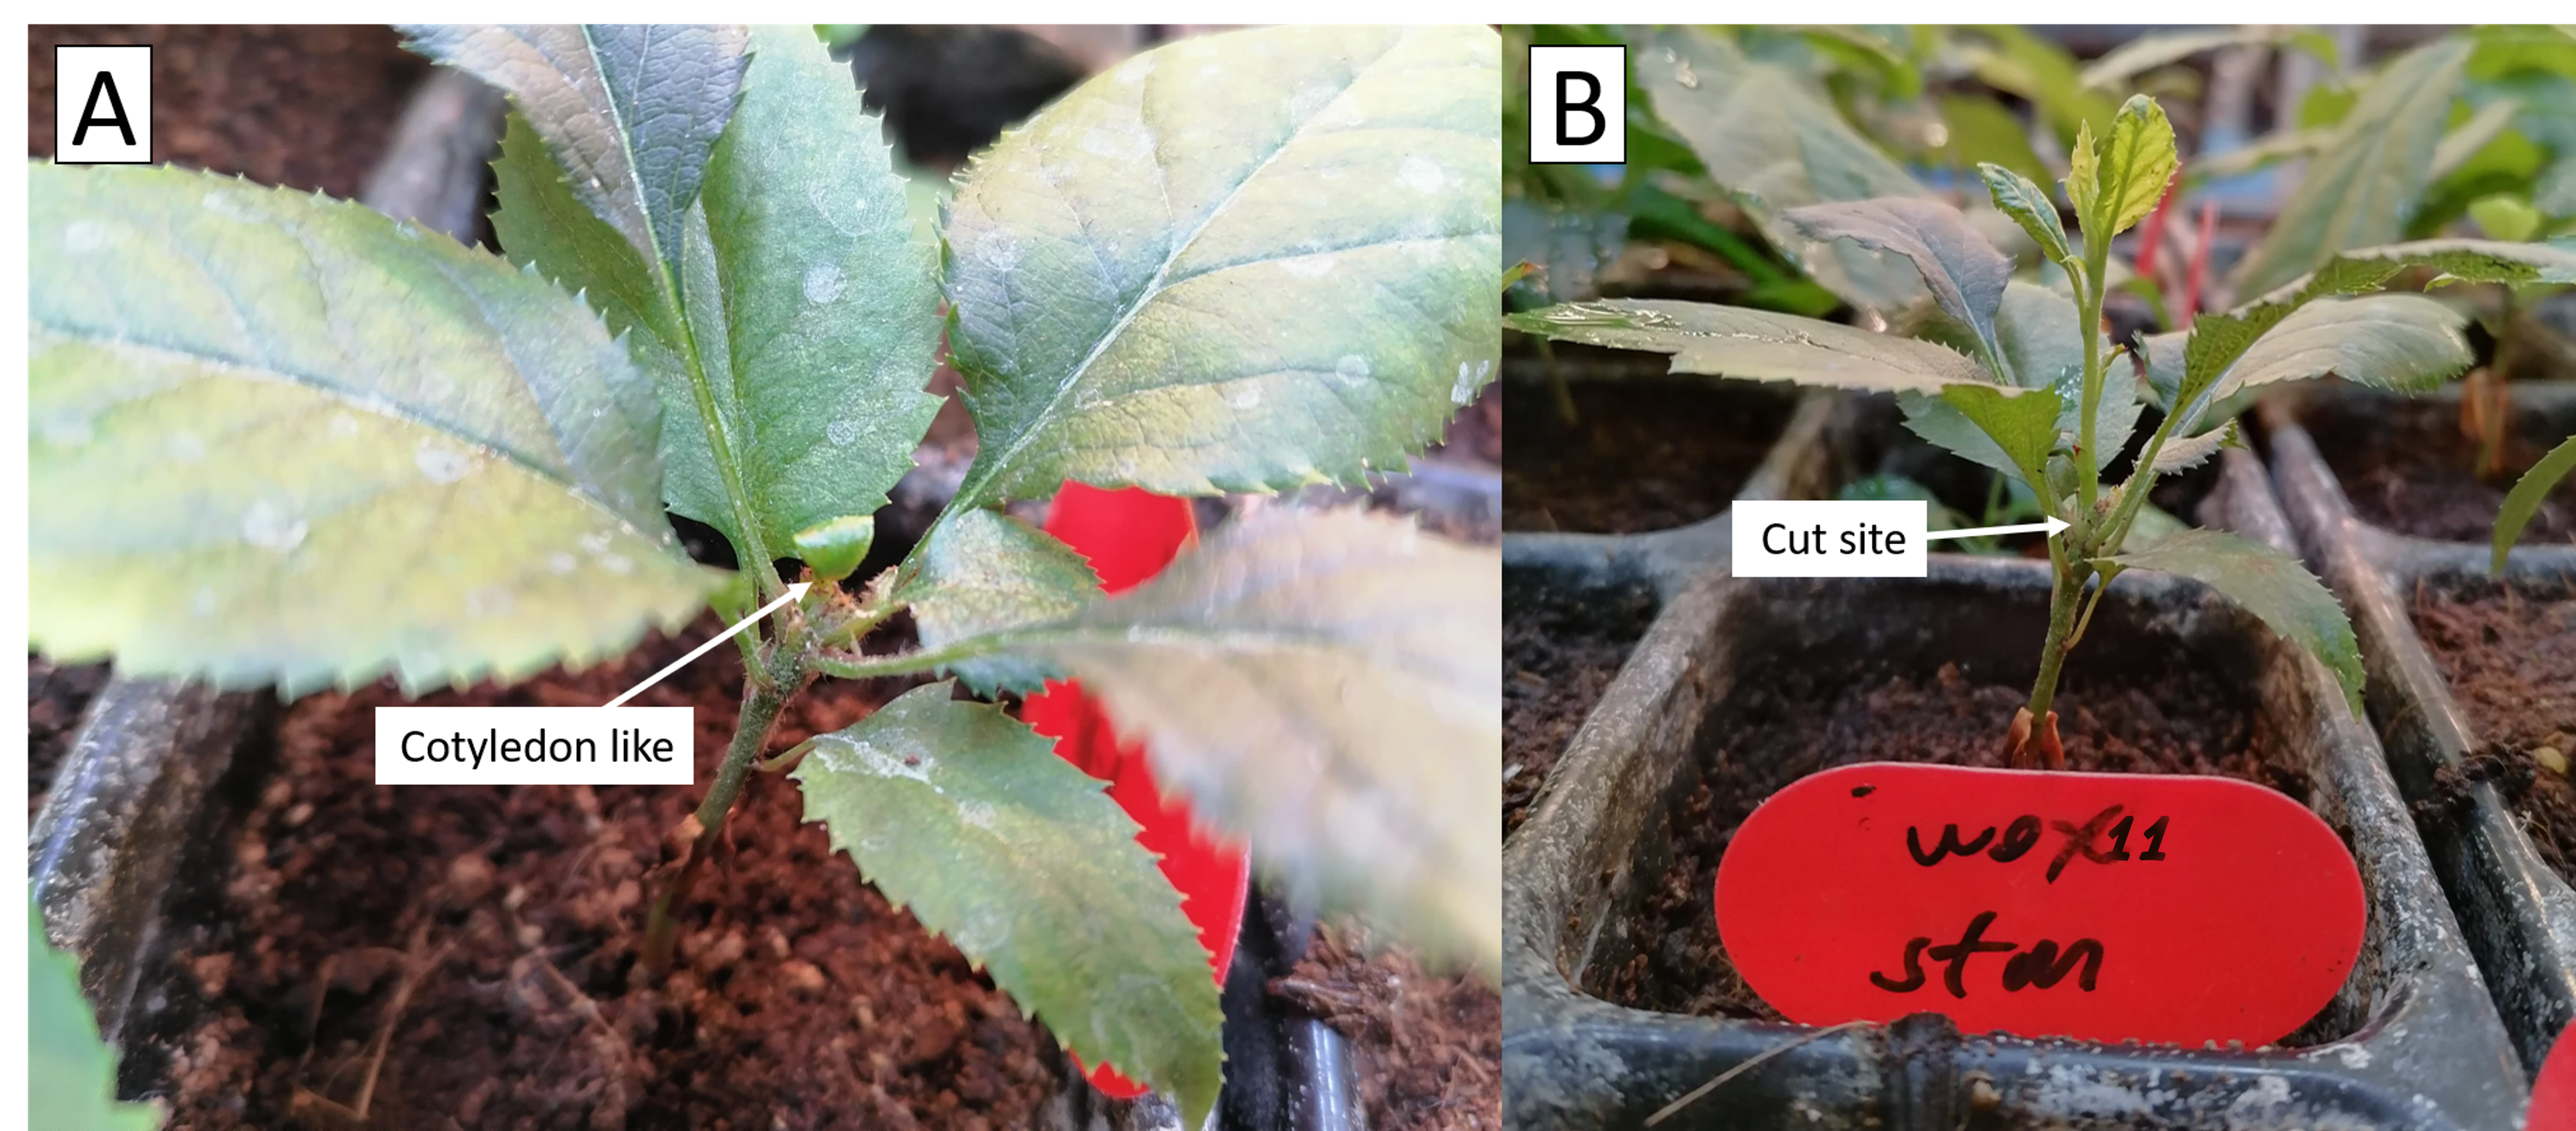
\includegraphics[width=1\linewidth]{wox-stm transformant3} 

}

\caption{Injection of A.tumefaciens into a stem cut of 4 apple Varieties. \newline{} \textbf{A.} Cotyledon like emerging from stem cut, two weeks post infection \textbf{B.} Shoot grow, three weeks post infection}\label{fig:wox-stm transformant}
\end{figure}

DNA was extracted from old leaf in the base of the plant and new leaf in
the shoot. A sequence from the T-DNA cassette that is part of the Cas9
gene was amplified with PCR reaction for the validation of T-DNA
integration in the genome. The PCR products was loaded in agarose gel
and run in electrophoresis bath. After that the gel was photographed on
a UV-light table. For posotive control the transformation plasmid
(pTRANS WOX11-STM) was used and for negative control the PCR stock
without DNA (Cas9 stock) was used. A band was observed in the new leaf
sample in the expected length, as seen in the positive control sample.
To validate that the DNA extraction was successful, a sequence from the
actin gene was amplified using PCR reaction and was anelyzed too by
agarose gel electrophoresis. For negative control the PCR stock without
DNA (Actin stock) was used (Figure \ref{fig:Cas9 gene in transformant}).

\begin{figure}[h]

{\centering \includegraphics[width=0.8\linewidth]{WOX-STM transformant Cas9+Actin3} 

}

\caption{Cas9 and actin validation using PCR. The products analysis by agarose gel electrophoresis. \newline{} \textbf{A.} T-DNA cassette validation with Cas9 primers \textbf{B.} DNA validation with actin primers}\label{fig:Cas9 gene in transformant}
\end{figure}

Both alleles of the S-RNase gene (S2 and S3) was amplified and sent for
sequencing for mutation analysis. No mutation was observed.

\hypertarget{drs-experiment-1}{%
\subsubsection{DRs experiment}\label{drs-experiment-1}}

Assessment of DRs for shoot induction in apple plants is preformed with
all constructs (Table \ref{tab:S-RNase Constracts}), on 4 apple
varieties (Figure \ref{fig:Agro-injection}) and with 11 repetitions per
construct. Out of 352 plants infected, 4 de-novo shoot regeneration was
observed, 3 of them are Pink-lady variety and the 4'th is Starking.
Shoot regeneration was observed after 1 week only. (Figure
\ref{fig:New transformant}).

\begin{figure}[h]

{\centering \includegraphics[width=0.8\linewidth]{Transformant2 results} 

}

\caption{Pink lady shoot regeneration. \newline{} \textbf{A.} and \textbf{B.} Grafting and cotyledone like appearance}\label{fig:New transformant}
\end{figure}

\hypertarget{scale-up-experiment-1}{%
\subsubsection{Scale-up experiment}\label{scale-up-experiment-1}}

At the scale up experiment about 800 seeds were planted, and as much as
400 plants were infected with 2 of the most promising plasmids and 1
control plasmid. As a result of disease infection that was spread on the
plants (Powdery mildew and Aphids), no phenotype as result of the
treatment was observed.

\hypertarget{high-humidity-experiment-1}{%
\subsubsection{High humidity
experiment}\label{high-humidity-experiment-1}}

At the high humidity experiment about 500 seeds were planted in a 300 ml
containers on sterile soil. The objective is to exclode any variables
from the enviroment and maintain moisture for the cells that exposed to
air in the proccess. Unfortunately, no shoot regeneration was observed.

\hypertarget{poplar-infections-1}{%
\subsubsection{Poplar infections}\label{poplar-infections-1}}

No phenotype as result of the treatment was observed.

\hypertarget{identification-of-new-trascription-factors-that-are-development-regulators-in-poplar}{%
\subsubsection{Identification of new trascription factors that are
development regulators in
poplar}\label{identification-of-new-trascription-factors-that-are-development-regulators-in-poplar}}

After several experiments in apples and poplar plants with the most
known DRs, the results were mixed and insufficient for further analysis.
We decided to try and identify new transcriptional factors that are more
representative of the tissue in question, shoot development. Therefore,
tissue specific transcriptome data was analyzed including shoot-tip
transcriptome. We found that from the WUSHCEL-related family, WOX1 was
by far the most expressed in shoot-tip in comparison to other tissues
(Figure \ref{fig:RNA-seq}).

\begin{figure}[h]

{\centering \includegraphics[width=0.8\linewidth]{Developing-noval-methods-for-gene-editing-in-trees_files/figure-latex/RNA-seq-1} 

}

\caption{WOX1 expression by the RNA-seq analysis}\label{fig:RNA-seq}
\end{figure}

\hypertarget{validation-of-the-rna-seq-analysis-with-real-time-quantitive-pcr-rt-qpcr-1}{%
\subsubsection{Validation of the RNA-seq analysis with real-time
quantitive PCR
(RT-qPCR)}\label{validation-of-the-rna-seq-analysis-with-real-time-quantitive-pcr-rt-qpcr-1}}

In most RT-qPCR expiraments, the samples are from the same tissue and
the only difference is a certine treatment (water salinity, gene
expression etc.). Therefor it is easy to choose an house-kipping gene to
act as a normalizer. In our case study, the samples are different
tissues, which differ in many biological pathways. At first, we tried to
use the most recognized house-keeping gene, Actin-7. The results showed
too much varience in the expression, so we went and looked in the
RNA-seq result for the most unchanged genes across all tissues and chose
2 genes, Serine/threonine-protein phosphatase PP2A-4 catalytic subunit
and E3 ubiquitin ligase. Further search in similar studies lead us to
investigate the genes PP2A-2 and U6 snRNA.

For further comparison, we anelyzed the RT-qPCR results dedpite the
normalizer inconsistatncy. (Figures \ref{fig:qPCR}))

\begin{figure}[H]

{\centering \includegraphics[width=1\linewidth]{Developing-noval-methods-for-gene-editing-in-trees_files/figure-latex/qPCR-1} 

}

\caption{WOX1 expression by the RT-qPCR with different normalizers. CV referse to the coefficient of variation and it represent a score for the amount in which the normalizer expressed consistently between the different tissues, measured as the standard deviation divided by the average expression. As the CV get smaller, the expression is more uniform.}\label{fig:qPCR}
\end{figure}

\hypertarget{conclusions}{%
\section{Conclusions}\label{conclusions}}

Food security is one of the major challenges facing humanity in the 21st
century (FAO 2011), especially in light of forecasts regarding climate
change and population growth. Cereals are staple crops and account for
as much as 44\% of all agriculture land use for food production
\href{https://ourworldindata.org/grapher/global-agricultural-land-use-by-major-crop-type}{(AREA
USED FOR PRODUCTION (FAO 2017))}. Cereal cultivars are annual plant and
as such are more prone to be effected by change in irrigation and
overall climate patterns(Shiferaw et al. 2014). In contrast, Trees,
especially fruit trees in the context of food production, are more
resilient to changes in the environment as a result of their strong and
deep roots. Consequently trees serves a vital role as a source for food
security. To date, fruit trees only serves a small part of the overall
food production. For trees to reach their full potential as staple crop
in many parts of the world, crop improvement methods need to be more
robust. Genetic engineering and especially genome editing methods with
the use of CRISPR/Cas9 technology have that potential. For those methods
to be adopted, they need to fulfill cretin criteria such as, speed, ease
of execution, cheap and minimal preliminary knowledge required. The most
common used method for crop improvement by genetic engineering is
agrobacterium-mediated transformation that is preformed on ex-plant in
sterile environment on tissue culture medium. Many researchers combined
that technology with CRISPR/Cas9 by integrating the Cas9 DNA sequence as
part of the agrobacterium T-DNA cassette. This method takes several
month at least to get from soil-grown wild type plant to soil-grown
transformant one, it takes very skilled personal to preform and require
preliminary knowledge in specific growth medium per cultivar.

In planta transformation is much desirable goal. In pursuing that
objective, Zhang et al.(Zhang et al. 2017) developed a new method for
plant transformation, that mimicks the work in tissue culture, but in
planta. In that method, rather than grow the whole plant in a sterile
envoriment on an agar medium, the researchers created micro enviroment
on an inner tissue section of the plant. It was done by cutting a stam
of a young pommelo plant, and enclosing it using a tube and parafilm.
The tube is than filled with a liquid growth medium containing
antibiotics and hormones (Figure \ref{fig:Pommelo}). Few seccess was
shown with that method, it holds several advantages over tissue colture
methods such as needs less time and labor cost, requires less equipments
and less strict experiment conditions and less skilled personal. but as
the design suggests, several of the drawbacks in tissue colture methods
are present here too, like the need for hormones and antibiotiotics.

Maher et al.(Maher et al. 2020) developed novel method for plant gene
editing by introducing DRs into the cell as well as CRISPR/Cas9 and
sgRNA, with the use of agrobacterium on soil-grown plants. In that way,
the phenotype formed by the transformation is de-novo shoot induction as
well as knockout in the gene of interest. This method have the potential
to remove the need entirely of tissue culture and enable gene editing in
planta. Furthermore, shoot regeneration is a direct result of the
transformation, therefor no induction with hormones or selection with
antibiotics is required in contrast to the work of Zhang et al.(Zhang et
al. 2017). In their work, to show de-novo shoot induction, the vector
was introduced to the location of axillary bud right after it was
surgically removed (Figure \ref{fig:Bud_Excision}). New shoot was formed
when the right combination of DRs was introduced, but in most cases it
was deformed as a result of the unregulated over expression of the DRs.

In this work we attempted to implement this novel transformation method,
on apple and poplar plants as the first trees used for this method. The
potential of this method is sound and in trees it is even more striking
when compared with traditional methods. Poplar tree was chosen as a
model tree and apple tree was chosen because of its commercially
importance. Also, a major set back in apple plantation is its
self-incompatibility, which means that new plantations need to be
vegetative reproduced mainly by cuttings and grafts. In apples S-RNase
is one of the key mechanisms that regulates self-incompatibility and as
such can serve a suited target for gene editing (Del Duca et al. 2019).
Therefor, the target gene of interest in this work is the apple's
S-RNase, if knocked out will have notable commercially importance, as
the first self-compatible apple variety. In poplar the target gene was
PDS because it is a well established reporter gene for the verification
of gene knockout.

In our work, we tried three different introduction of the agrobacterium
to the plant, pressure injection to the leaf surface, injection to leaf
vains and injection to stem cut. Similar to the method described by
Zhang et al., our result was in favor of the latter (Figure
\ref{fig:Pommelo}). In comparison to Maher et al.~that describe the work
on \emph{Nicotiana benthamiana} and also mentioned work on tomato,
potato and grape, we attempted to implement the method on apple and
poplar trees. Another result different in comparison to their work, the
new shoot formed on the top of the stem was not deformed (Figure
\ref{fig:Deform_benthamiana}), possibly as a result of the nature of the
growth, mimicking the natural shoot apical meristem, and the apical
control with all its hormone flux involve in the process.

In the infection methods experiment only 1 plant was infected with each
plasmid with the method described and later on shown promise results in
de-novo shoot regeneration. Although regenerative plants was clearly
observed, no mutation was found as a result of the Cas9 activity.
Further investigation is required in the subject for more conclusive
results, Therefor DRs experiment was preformed, with more repetitions
and wider range of apple varieties.

In the DRs experiment 352 plants infected, out of 44 infected with
\emph{WOX11}-\emph{STM}, 4 regenerate new shoot from the cut site. In
the infection methods experiment, the cut site was not covered. After
reviewing the work of (Zhang et al. 2017), a decision was made to use
parafilm for better moister maintenance.

In the scale-up experiment, both parafilm and aluminum foil was used to
cover the stem cut for kipping dark and moist environment. The Dark
environment is crucial in the first 48 hours for the agrobacterium
infection. Unfortunately, as a result of disease spread, no phenotype
was observed.

To increase the possibility of infection success, the next seeds were
grown under aseptic conditions, on soil. And were kept in a high
humidity environment. No shoot regeneration formed in that case too.

To further attempt and increase the frequency of de-novo shoot
formation, we pursue the identification of new trascription factors that
are development regulators in trees and parhapse, under the right
conditions, would act as a master regulators. Fortunatly, in 2017 the
\href{https://genome.jgi.doe.gov/portal/PoptreSequencing_FD/PoptreSequencing_FD.info.html}{\textbf{DOE
Joint Genome Institute}} (Grigoriev et al. 2012) sequenced the
\emph{Populus tremula x alba} INRA717-IB4 transcriptome. With that
dataset available, we could analyse the transcription profile per
tissue, and highlight certine genes that holds strong correlation to the
development of shoot. In our analysis we found that out of the
WUSCHEL-related homeobox (WOX) gene family, \emph{WOX1} had the
strongest correlation for shoot formation. That finding correspond to
the findings mentioned in Tvorogova et al's. review (Tvorogova et al.
2021), there \emph{WOX1} found to regulate auxin response. This can be
realized since many of the genes whose expression is affected by WOX1
are involved in signaling pathways, transport, and synthesis of auxin.
Furthermore,~after~narrowing~the~results~only~to~those~genes~that~are~at~least~an~order~of~magnitude~shoot~specific~over~all~tissues,~WOX1~came~in~8'th~position~out~of~85~genes.

With strong corelation to our results of regeneration with the
combination of genes \emph{WOX11}-\emph{STM} and \emph{WUS2}-\emph{STM},
It has been shown that in the regulation of SAM, STM and WUS act in
parallel, and they are necessary for the normal expression of each other
(Tvorogova et al. 2021). This insight can also explain the non-deformed
shoot formation we observe in contrast to Maher et al's.(Maher et al.
2020) findings.

\emph{WOX11} known primarily as regulators of callus formation and
development of adventitious roots, although it has been shown to be
involved in other types of regeneration, such as shoot regeneration and
somatic embryogenesis. For example, the positive effect of PtWOX11 on
shoot regeneration in \emph{Populus alba x glandulosa} has been shown
(Liu et al. 2018).

To validate our RNA-seq analisys, we extracted total RNA from similar
tissues as the DOE's dataset (excluding callus, since it does not acure
in natural growth). Then we run RT-qPCR analisys on the expression of
\emph{WOX1} with varius normalizer genes. Since the expression profile
of the different tissues vary massivly, it has been hard to find an
appropriate normalizer gene whose expression remains homogeneousness
between the tissues. Despite that, we can still see the over all trend
in which it does seems that as the coefficient of variation (CV) get
smaller, the results of the RT-qPCR become more similar to the RNA-seq
results (Figure \ref{fig:qPCR}).

\hypertarget{acknowledgements}{%
\section{Acknowledgements}\label{acknowledgements}}

\hypertarget{supplementary-information}{%
\section{Supplementary information}\label{supplementary-information}}

\href{https://htmlpreview.github.io/?https://raw.githubusercontent.com/BenSiv/PopAT-expression-analysis/main/PopAT_Expression.html}{Analysis
code link.}

\begin{figure}[h]

{\centering \includegraphics[width=1\linewidth]{Bud excision} 

}

\caption{Surgical removal of the axillary bud and injection of vector for de-novo shoot induction (Maher et al. 2020)}\label{fig:Bud_Excision}
\end{figure}
\begin{figure}[h]

{\centering \includegraphics[width=1\linewidth]{Deform benthamiana PDS} 

}

\caption{Abnormal shoot regeneration formation as a result of DR over-expression (Maher et al. 2020)}\label{fig:Deform_benthamiana}
\end{figure}
\begin{figure}[H]

{\centering \includegraphics[width=0.8\linewidth]{Pommelo transformation} 

}

\caption{Agrobacterium-mediated in planta transformation for Citrus maxima. \textbf{a.} Three to four week old C. maxima seedlings. \textbf{b.} Decapitated C. maxima seedlings. \textbf{c.} Agrobacterium infection. \textbf{d.} Agrobacterium infected seedlings with wounds wrapped with Parafilm. \textbf{e.} Dark incubation during co-culture. \textbf{f.} sprouted bud from newly formed callus. \textbf{g.} sprouted buds from xylem. \textbf{h.} regenerated shoots four weeks after transformation. \textbf{i.} regenerated shoots three months after transformation. (Zhang et al. 2017)}\label{fig:Pommelo}
\end{figure}

\hypertarget{references}{%
\section*{References}\label{references}}
\addcontentsline{toc}{section}{References}

\hypertarget{refs}{}
\begin{CSLReferences}{0}{0}
\leavevmode\vadjust pre{\hypertarget{ref-Barrangou1709}{}}%
Barrangou R, Fremaux C, Deveau H, Richards M, Boyaval P, Moineau S,
Romero DA, Horvath P. 2007. {CRISPR Provides Acquired Resistance Against
Viruses in Prokaryotes}. Science. 315:1709--1712.

\leavevmode\vadjust pre{\hypertarget{ref-Chandrasegaran1996}{}}%
Chandrasegaran S. 1996. {Hybrid restriction enzymes : Zinc finger
fusions to Fok I cleavage domain}. Proceedings of the National Academy
of Sciences. 93:1156--1160.

\leavevmode\vadjust pre{\hypertarget{ref-Christian2010}{}}%
Christian M, Cermak T, Doyle EL, Schmidt C, Zhang F, Hummel A, Bogdanove
AJ, Voytas DF. 2010. {Targeting DNA double-strand breaks with TAL
effector nucleases}. Genetics. 186:756--761.

\leavevmode\vadjust pre{\hypertarget{ref-Cermak2017}{}}%
Čermák T, Curtin SJ, Gil-Humanes J, Čegan R, Kono TJY, Belanto JJ,
Starker CG, Mathre JW, Greenstein RL, Daniel F, et al. 2017. {A
multipurpose toolkit to enable advanced genome engineering in plants}.
Plant Cell. 29:1196--1217.

\leavevmode\vadjust pre{\hypertarget{ref-davey2005plant}{}}%
Davey MR, Anthony P, Power JB, Lowe KC. 2005. {Plant protoplasts: Status
and biotechnological perspectives}. Biotechnology Advances. 23:131--171.

\leavevmode\vadjust pre{\hypertarget{ref-DelDuca2019}{}}%
Del Duca S, Aloisi I, Parrotta L, Cai G. 2019. {Cytoskeleton,
transglutaminase and gametophytic self-incompatibility in the Malinae
(Rosaceae)}. International Journal of Molecular Sciences. 20:1--11.

\leavevmode\vadjust pre{\hypertarget{ref-Enciso-Rodriguez2019}{}}%
Enciso-Rodriguez F, Manrique-Carpintero NC, Nadakuduti SS, Buell CR,
Zarka D, Douches D. 2019. {Overcoming self-incompatibility in diploid
potato using CRISPR-cas9}. Frontiers in Plant Science. 10:1--12.

\leavevmode\vadjust pre{\hypertarget{ref-Ericksen2009}{}}%
Ericksen PJ, Ingram JSI, Liverman DM. 2009. {Food security and global
environmental change: emerging challenges}. Environmental Science and
Policy. 12:373--377.

\leavevmode\vadjust pre{\hypertarget{ref-FAO2011}{}}%
FAO. 2011. {in the 21 st Century}. {[}place unknown{]}.

\leavevmode\vadjust pre{\hypertarget{ref-FAO2020a}{}}%
FAO. 2020. {Food Security and Nutrition in the World. Transofrmin food
systems for affordable healthy diets}. {[}place unknown{]}.

\leavevmode\vadjust pre{\hypertarget{ref-Garrity2010}{}}%
Garrity DP, Akinnifesi FK, Ajayi OC, Weldesemayat SG, Mowo JG,
Kalinganire A, Larwanou M, Bayala J. 2010. {Evergreen Agriculture: A
robust approach to sustainable food security in Africa}. Food Security.
2:197--214.

\leavevmode\vadjust pre{\hypertarget{ref-GasiunasE2579}{}}%
Gasiunas G, Barrangou R, Horvath P, Siksnys V. 2012. {Cas9 crRNA
ribonucleoprotein complex mediates specific DNA cleavage for adaptive
immunity in bacteria}. Proceedings of the National Academy of Sciences.
109:E2579-----E2586.

\leavevmode\vadjust pre{\hypertarget{ref-Gibson2009}{}}%
Gibson DG, Young L, Chuang RY, Venter JC, Hutchison CA, Smith HO. 2009.
{Enzymatic assembly of DNA molecules up to several hundred kilobases}.
Nature Methods. 6:343--345.

\leavevmode\vadjust pre{\hypertarget{ref-Grigoriev2012}{}}%
Grigoriev IV, Nordberg H, Shabalov I, Aerts A, Cantor M, Goodstein D,
Kuo A, Minovitsky S, Nikitin R, Ohm RA, et al. 2012. {The Genome Portal
of the Department of Energy Joint Genome Institute}. Nucleic Acids
Research. 40:26--32.

\leavevmode\vadjust pre{\hypertarget{ref-Rosenzweig2001}{}}%
Iglesius A, Epstein PR, Chivian E, Rosenzweig C, Iglesias A, Yang XB,
Epstein PR, Chivian E. 2001. {Implications for food production, plant
diseases, and pests}. Global Change and Human Health. 2:90--104.

\leavevmode\vadjust pre{\hypertarget{ref-Indra1972}{}}%
Indra K, Vimla V. 1972. {Totipotecy and embryogenesis in plant cell and
tissue cultures}. In vitro. 8.

\leavevmode\vadjust pre{\hypertarget{ref-Jinek2012}{}}%
Jinek M, Chylinski K, Fonfara I, Hauer M, Doudna JA, Charpentier E.
2012. {A programmable dual-RNA-guided DNA endonuclease in adaptive
bacterial immunity}. Science. 337:816--821.

\leavevmode\vadjust pre{\hypertarget{ref-Kaeppler2000}{}}%
Kaeppler SM, Kaeppler HF, Rhee Y. 2000. {Epigenetic aspects of
somaclonal variation in plants}. Plant Molecular Biology. 43:179--188.

\leavevmode\vadjust pre{\hypertarget{ref-Linden2015}{}}%
Linden PVD, Office M. 2015. {Climate Change 2007 : Impacts , Adaptation
and Vulnerability INTERGOVERNMENTAL PANEL ON CLIMATE CHANGE Climate
Change 2007 : Impacts , Adaptation and Vulnerability Working Group II
Contribution to the Intergovernmental Panel on Climate Change Summary
for }.

\leavevmode\vadjust pre{\hypertarget{ref-Liu2018a}{}}%
Liu B, Zhang J, Yang Z, Matsui A, Seki M, Li S, Yan X, Kohnen MV, Gu L,
Prasad K, et al. 2018. {PtWOX11 acts as master regulator conducting the
expression of key transcription factors to induce de novo shoot
organogenesis in poplar}. Plant Molecular Biology. 98:389--406.

\leavevmode\vadjust pre{\hypertarget{ref-Maher2020}{}}%
Maher MF, Nasti RA, Vollbrecht M, Starker CG, Clark MD, Voytas DF. 2020.
{Plant gene editing through de novo induction of meristems}. Nature
Biotechnology. 38:84--89.

\leavevmode\vadjust pre{\hypertarget{ref-Mukeshimana2013}{}}%
Mukeshimana G, Ma Y, Walworth AE, Song G qing, Kelly JD, Song G qing,
Kelly JD. 2013. {Factors influencing regeneration and Agrobacterium
tumefaciens-mediated transformation of common bean (Phaseolus vulgaris
L.)}. Plant Biotechnology Reports. 7:59--70.

\leavevmode\vadjust pre{\hypertarget{ref-OBrien2011}{}}%
O'Brien JA, Lummis SCR. 2011. {Nano-biolistics: A method of biolistic
transfection of cells and tissues using a gene gun with novel
nanometer-sized projectiles}. 11.

\leavevmode\vadjust pre{\hypertarget{ref-Qaim2013}{}}%
Qaim M, Kouser S. 2013. {Genetically Modified Crops and Food Security}.
PLoS ONE. 8:1--7.

\leavevmode\vadjust pre{\hypertarget{ref-Rakoczy-Trojanowska2002}{}}%
Rakoczy-Trojanowska M. 2002. {Alternative methods of plant
transformation - A short review}. Cellular and Molecular Biology
Letters. 7:849--858.

\leavevmode\vadjust pre{\hypertarget{ref-Rasmussen2017}{}}%
Rasmussen SK, Kumar Mall T, Duraialagaraja S, Agrawal PK, Yadava P,
Abhishek A, Singh R, Singh I, Kaul T, Pattanayak A. 2017. {Advances in
Maize Transformation Technologies and Development of Transgenic Maize}.
Front Plant Sci. 7:1949.

\leavevmode\vadjust pre{\hypertarget{ref-Schouten2007}{}}%
Schouten HJ, Jacobsen E. 2007. {Are mutations in genetically modified
plants dangerous?} Journal of Biomedicine and Biotechnology. 2007:2--4.

\leavevmode\vadjust pre{\hypertarget{ref-Shalem84}{}}%
Shalem O, Sanjana NE, Hartenian E, Shi X, Scott DA, Mikkelsen TS, Heckl
D, Ebert BL, Root DE, Doench JG, Zhang F. 2014. {Genome-Scale
CRISPR-Cas9 Knockout Screening in Human Cells}. Science. 343:84--87.

\leavevmode\vadjust pre{\hypertarget{ref-Shewry2008149}{}}%
Shewry PR, Jones HD, Halford NG. 2008. {Plant biotechnology: Transgenic
crops}. Advances in Biochemical Engineering/Biotechnology. 111:149--186.

\leavevmode\vadjust pre{\hypertarget{ref-Shiferaw2014}{}}%
Shiferaw B, Tesfaye K, Kassie M, Abate T, Prasanna BM, Menkir A. 2014.
{Managing vulnerability to drought and enhancing livelihood resilience
in sub-Saharan Africa: Technological, institutional and policy options}.
Weather and Climate Extremes. 3:67--79.

\leavevmode\vadjust pre{\hypertarget{ref-Taylor2002}{}}%
Taylor G. 2002. {Populus: Arabidopsis for forestry. Do we need a model
tree?} Annals of Botany. 90:681--689.

\leavevmode\vadjust pre{\hypertarget{ref-TesterMarkandLangridge2010}{}}%
Tester, Mark and Langridge P. 2010. {Breeding Technologies to Increase}.
Science. 818:818--822.

\leavevmode\vadjust pre{\hypertarget{ref-Tvorogova2021}{}}%
Tvorogova VE, Krasnoperova EY, Potsenkovskaia EA, Kudriashov AA, Dodueva
IE, Lutova LA. 2021. {What Does the WOX Say? Review of Regulators,
Targets, Partners}. Molecular Biology.

\leavevmode\vadjust pre{\hypertarget{ref-Undervisningsministeriet2014}{}}%
Undervisningsministeriet. 2014. {Enhanced Reader.pdf}. :1.

\leavevmode\vadjust pre{\hypertarget{ref-Vinceti2013}{}}%
Vinceti B, Termote C, Ickowitz A, Powell B, Kehlenbeck K, Hunter D.
2013. {The contribution of forests and trees to sustainable diets}.
Sustainability (Switzerland). 5:4797--4824.

\leavevmode\vadjust pre{\hypertarget{ref-Zhang2006}{}}%
Zhang X, Henriques R, Lin SS, Niu QW, Chua NH. 2006.
{Agrobacterium-mediated transformation of Arabidopsis thaliana using the
floral dip method}. Nature Protocols. 1:641--646.

\leavevmode\vadjust pre{\hypertarget{ref-Zhang2017}{}}%
Zhang Y yan, Zhang D min, Zhong Y, Chang X jun, Hu M lun, Cheng C zhen.
2017. {A simple and efficient in planta transformation method for
pommelo (Citrus maxima) using Agrobacterium tumefaciens}. Scientia
Horticulturae. 214:174--179.

\end{CSLReferences}

\end{document}
